\chapter*{Your \sectionsovs drip}
\textit{``Does \sovs have a uniform?''} \textit{``Do you think she'll go for this \textit{dobok}/\textit{dashiki}/\textit{toque} combo?''} \footnote{Sure... You're good!} \textit{``Do you think the females will digg this forrest green and sunflower yellow track suit/skull cap mix?''} \footnote{I don't know man... sounds a little sketchy. Maybe. Try not to be fat}\\
Unfortunately, hitting the dance floor isn't as simple as just rolling out of bed and going to the club in your jammies, but will involve such boring practicalities as picking out clothes to wear that won't have the doormen ``randomly'' picking you out at the entrance and preemptively beating your silly-looking ass with a nightstick. Good news is though, that in terms of \sovs, there are is no fashion police: you do you!\\
However, seeing as the music at most dancing venues is rather loud and your cauliflowered ears may not function the way they used to, you may want to find a non-verbal way to let your dance partner know that you are a \sovseneer \footnote{especially if you are a \dude in a country that enforces some kind of legislation against unprovoked acts of violence, letting \gal know that she is not liable to criminal charges if she punches you in the face, is hella \textbf{gentleman}}  and besides from tattooing \sovs on your extremeties, expressing it through your choice of clothing seems like the obvious idea. Now, I am no fashion guru. I would even go so far as to say, that given predicate $p$ such that $p(a,b)$ is \textit{true} for persons $a$ and $b$ \textit{iff.} $a$ knows more about fashion than $b$, it holds that 

\begin{equation*}
P(p(a_x, \pmb{Sunetiago} \; \pmb{Hansen}) \; is \; \pmb{true})) \geq 96.45\%, \; \forall \; a_x  \in  S_{10} 
\end{equation*}

where $S_{10}$ is the set consisting of human beings older than $10$ years of age.\\
Nonetheless, in the following I will provide some suggestions for inspiration to your \sovs-uniform. Whether the bouncers at the club will let you in and/or if they will get you beat up on the way to/from the club, I have no idea. The suggestions should mostly apply to both \dude and \gal, but please apply common sense. 

\newpage
\subsection*{Lower body}
Most clothing made for martial arts, is made with durability and flexibility in mind, so I suggest looking towards the martial arts for inspiration when it comes to finding appropriate \sovs leg-wear. You could repurpose the pants from your old \textit{Taekwondo} or \textit{Kong Fu} uniform, or if you feel like showing off your new tats and sturdy legs, you could go for the familiar \textit{Muay Thai} shorts. 

\vspace{10pt}

\begin{center}
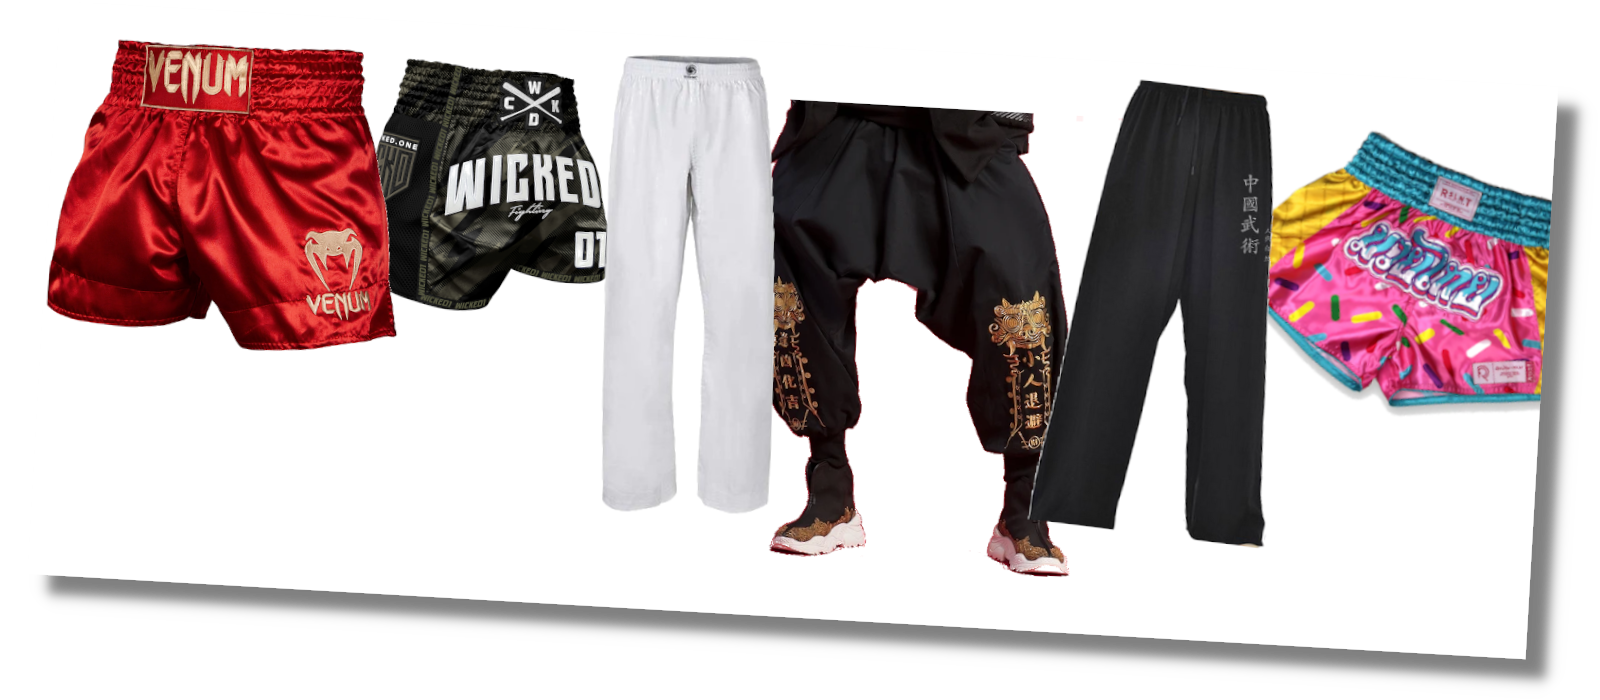
\includegraphics[scale=0.3]{03-Outro/lower-body-final}
\end{center}


\newpage
\subsection*{Upper body}
Do you remember the last time you went to a party in a shazzy Hawaii-shirt, and everyone was like: \textit{``OMG, that shirt is HORRIBLE!''}. No? That's because it has never happened, and that's because Hawaii shirts at dance parties are an evergreen. In general, I recommend looking towards the equator when picking out upper body wear for \sovsing. 

\vspace{10pt}

\begin{center}
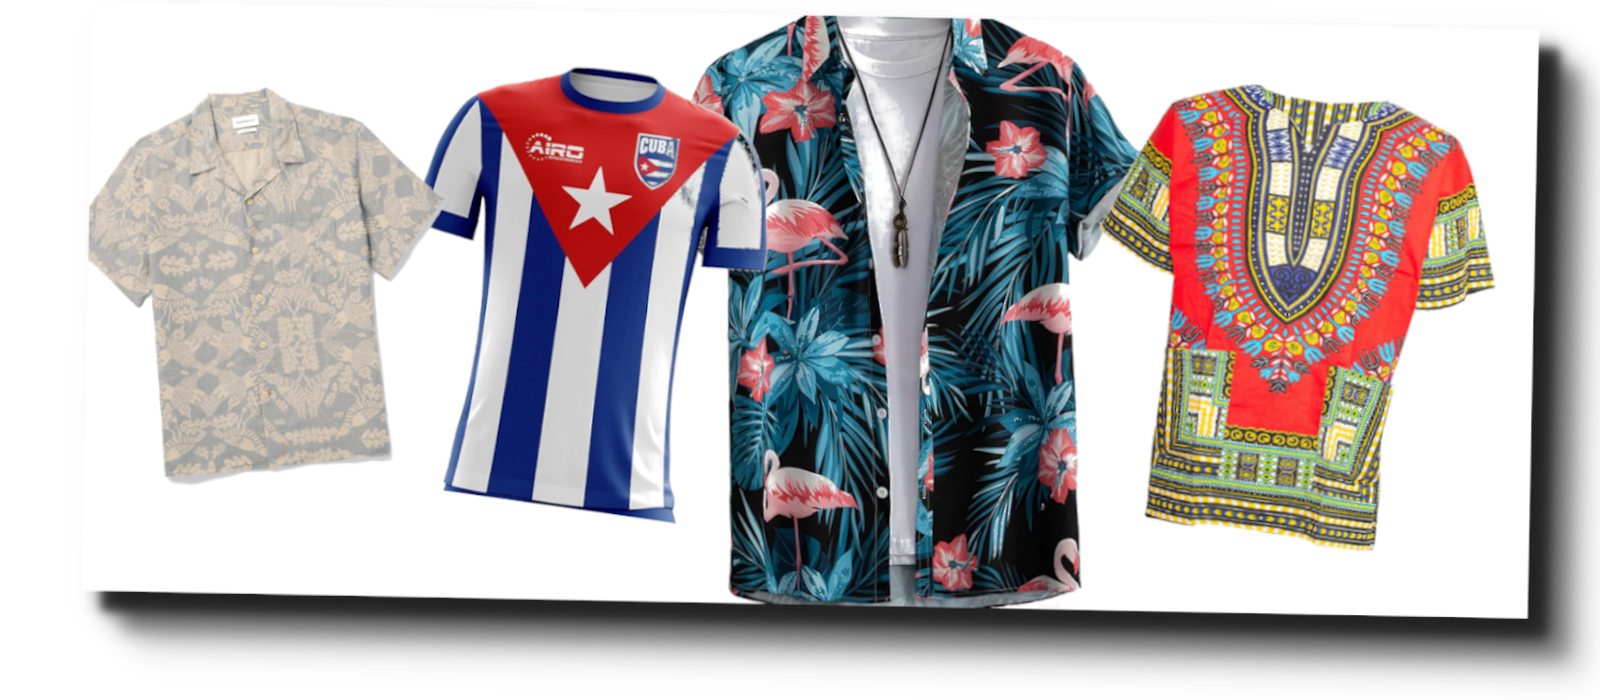
\includegraphics[scale=0.3]{03-Outro/upper-body-wear-final}
\end{center}

\vspace{10pt}

\newpage
\subsection*{Accessories}
I once, while driving a car, tuned into a radio program starring 2 metrosexuals talking about really expensive watches. I don't remember much from that show, but they seemed to make a great deal about \textit{accessorizing} your wardrobe. Personally, the only accessory I have ever  bought has been cufflinks \footnote{a friend of mine gifted me some expensive work-shirts he had become too fat to use himself, and for a while I was wondering what type of \textbf{\textit{absolute scoundrel}} gives away shirts without those sleeve buttons}, but I can totally see how there are some really cool ways to turn your regular clubbing wardrobe into genuine \sovs gear with just a couple of accessories.

\begin{center}
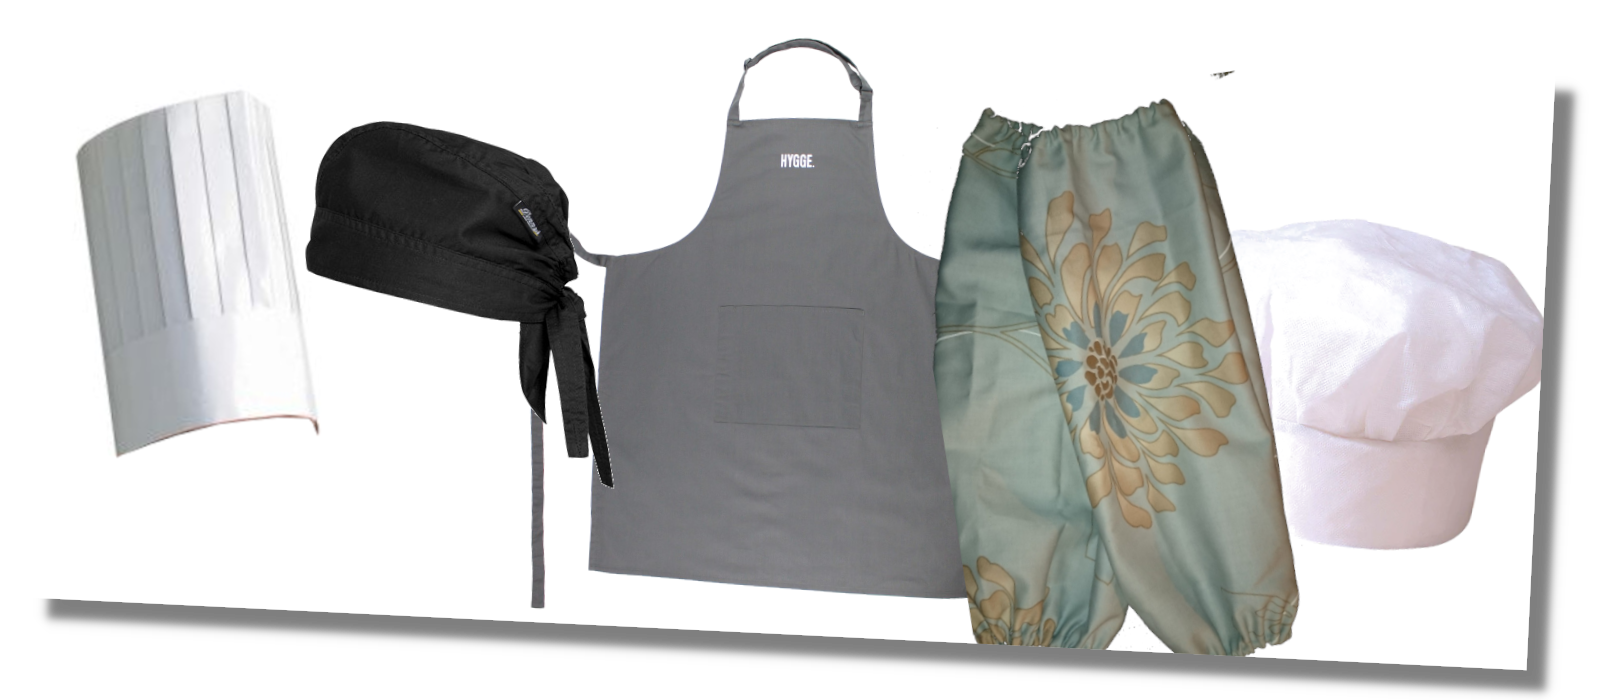
\includegraphics[scale=0.3]{03-Outro/accessories-final}
\end{center}
